\documentclass[12pt]{article}

\usepackage[margin=1in]{geometry} 
\usepackage[font=small,labelfont=bf]{caption}
\usepackage{mathtools}
\usepackage{titlesec}

\titleformat*{\section}{\large\bfseries}
\titleformat*{\subsection}{\bfseries}

\begin{document}

\begin{center}
    {\LARGE Machine Learning with Fetal Health dataset} \\[0.6cm]

    Marcus Lee \\
    \texttt{\small marcustutorial@hotmail.com} \\[0.3cm]

    \small \today
\end{center}

\begin{section}{Data Preparation / Cleaning}

 \subsection{Normalization}
 Since the features in the dataset has different scales, I applied a
 \textit{Normalize} filter with scale of 100, so every data falls on the
 range $[0, 100]$.

 \begin{center}
     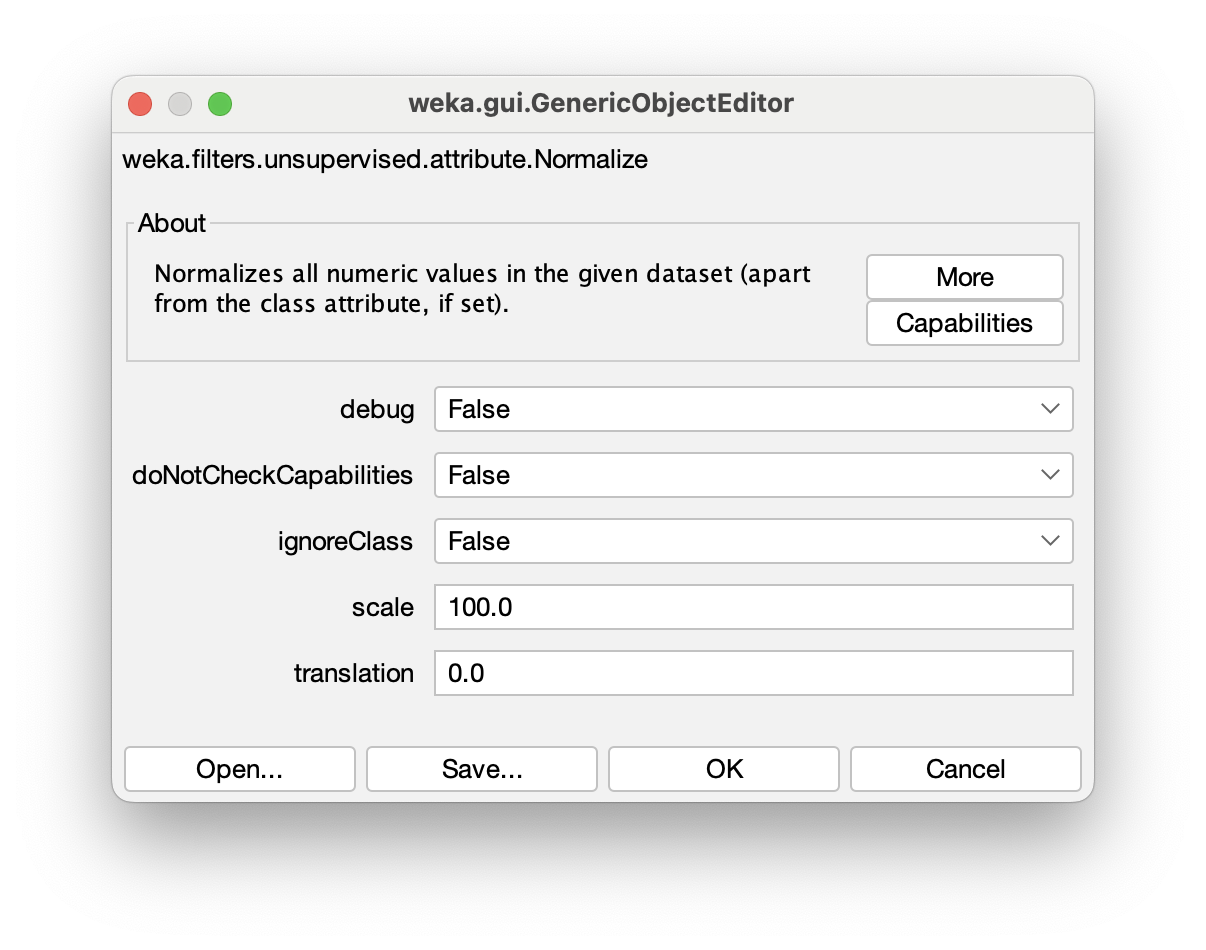
\includegraphics[width=8cm]{images/1_1_normalisation.png}
     \captionof{figure}{Normalization}
 \end{center}

 \subsection{Feature removal}
 Then I manually removed the feature \textit{severe\_decelerations} because
 it is mostly 0 except for once it is 0.001, and that could introduce noise.
\end{section}

\begin{section}{Classify with k-NN, Naive Bayes and Decision Tree}
 \subsection{Choosing the accuracy measures}
 The accuracy measures I chose is \textbf{F1-Measure}. This is due to the fact
 that F1-Measure is a combination of both precision and recall, it reflects
 the true positive rate and false positive rate of the classifiers' performance.
 Because of that this measure tells us a more complete picture of each classifier's
 pros and cons compared to other measures such as accuracy. Hence, it is easier for
 us to compare and determine the trade-offs between the classifiers. \\

 To clarify, Weka labels it as \texttt{F-Measure} but it is the same as F1-Measure
 because it uses harmonic mean ($\beta = 1$) in the calculation of:

 \begin{align*}
     F = \frac{(1 + \beta^2) \cdot Precision \cdot Recall}{\beta^2 \cdot Precision + Recall}
 \end{align*}

 \subsection{Discussion on the different accuracy values}
 By running the classifiers with default parameters by Weka, the results are as follows:

 \begin{center}
     \begin{tabular}{| c | c | c | c |}
         \hline
         \textbf{F1-Measure}       & \textbf{Naive Bayes} & \textbf{k-NN} & \textbf{Decision Tree} \\ [0.5ex]
         \hline
         \textbf{Normal}           & 0.900                & 0.955         & 0.958                  \\
         \hline
         \textbf{Pathologic}       & 0.603                & 0.860         & 0.936                  \\
         \hline
         \textbf{Suspect}          & 0.621                & 0.717         & 0.774                  \\
         \hline
         \hline
         \textbf{Weighted Average} & 0.837                & 0.915         & 0.931                  \\
         \hline
     \end{tabular}
     \captionof{table}{F1-Measure of each class and the weighted average}
 \end{center}

 The \textbf{weighted average} is the average of the F1-Measure of each class weighted by the number of instances in each class.
 The formula is as follows:

 \begin{center}
     $F1_{weighted} = \frac{F1_{normal} \times n_{normal} + F1_{pathologic} \times n_{pathologic} + F1_{suspect} \times n_{suspect}}{n_{normal} + n_{pathologic} + n_{suspect}}$
 \end{center}

 From the results above, Naive Bayes is the worst performing classifier and this is because
 the features in the dataset depends on each other for example, when there are lesser
 \textbf{accelerations}, there are also lesser \textbf{fetal\_movement} whereas Decision Tree
 performed the best with $0.931$ and k-NN being the close second with $0.915$.

 \subsection{Finding the optimal value of $k$ for k-NN}
 The table below shows the weighted average F1-Measure by running the k-NN classifier with odd values of $k$ from 1 to 15.

 \begin{center}
     \begin{tabular}{| c | c |}
         \hline
         \textbf{k} & \textbf{F1-Measure (weighted average)} \\ [0.5ex]
         \hline
         1          & 0.915                                  \\
         \hline
         3          & 0.907                                  \\
         \hline
         5          & 0.905                                  \\
         \hline
         7          & 0.899                                  \\
         \hline
         9          & 0.894                                  \\
         \hline
         11         & 0.889                                  \\
         \hline
         13         & 0.891                                  \\
         \hline
         15         & 0.889                                  \\
         \hline
     \end{tabular}
     \captionof{table}{F1-Measure of k-NN from $k = 1$ to $k = 15$}
 \end{center}

 From the results above, we can observe a downtrend as $k$ increases and the highest F1-Measure recorded is when
 $k = 1$. However, I would consider $k = 3$ to be the optimal value because generally overfits occur when $k=1$.
 In addition, I purposely skipped even number of $k$ to avoid ties.

 \subsection{Using 1/d weighting}
 Using only $k = 3$, I applied 1/d weighting to the k-NN classifier and the results are as follows:

 \begin{center}
     \begin{tabular}{| c | c |}
         \hline
         \textbf{F1-Measure (No distance weighting)} & \textbf{F1-Measure (Weight by 1/distance)} \\ [0.5ex]
         \hline
         0.907                                       & 0.913                                      \\
         \hline
     \end{tabular}
     \captionof{table}{F1-Measure of k-NN with 1/d weighting where $k = 3$}
 \end{center}

 Note that the F1-Measure above is the weighted average. From the results above, we do see a slight improvement
 by applying 1/d weighting to the k-NN classifier.

 \subsection{Using $k = 3$ and $k = 5$ fold-cross validation}
 The table below shows the weighted average F1-Measure by running the k-NN classifier with $k = 10$ (default),
 $k = 5$ and $k = 3$ fold-cross validation.

 \begin{center}
     \begin{tabular}{| c | c | c |}
         \hline
         \textbf{k fold-cross validation} & \textbf{F1-Measure (Weight by 1/distance)} \\ [0.5ex]
         \hline
         10                               & 0.913                                      \\
         \hline
         5                                & 0.912                                      \\
         \hline
         3                                & 0.908                                      \\
         \hline
     \end{tabular}
     \captionof{table}{F1-Measure of k-NN with varying k fold-cross validation}
 \end{center}

 From the results above, we can observe that the results does change with different value k fold-cross validation
 because when k fold-cross validation decreases, F1-Measure also decreases.
\end{section}

\begin{section}{Receiver operating characteristic (ROC) curves}
 \subsection{ROC Curves for the classification models}
 \subsubsection{Naive Bayes}

 \begin{center}
     \begin{minipage}{0.48\linewidth}
         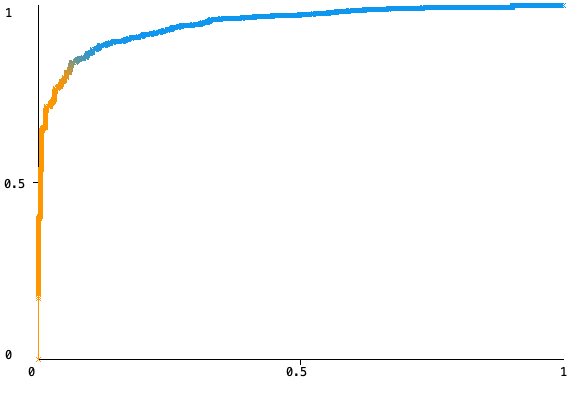
\includegraphics[width=8cm]{images/3_1_naive_bayes_normal.png}
         \captionof{figure}{Naive Bayes (Normal)}
     \end{minipage}
     \begin{minipage}{0.48\linewidth}
         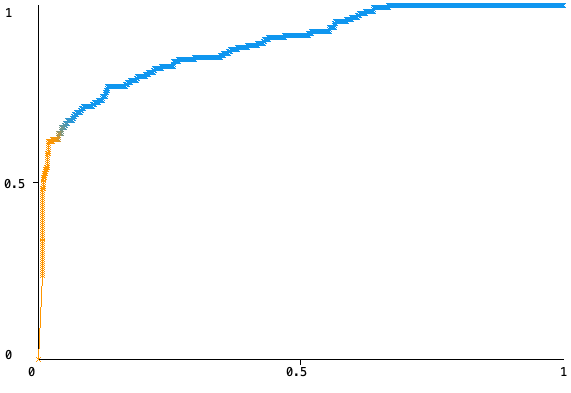
\includegraphics[width=8cm]{images/3_1_naive_bayes_pathological.png}
         \captionof{figure}{Naive Bayes (Pathological)}
     \end{minipage}
     \begin{minipage}{0.48\linewidth}
         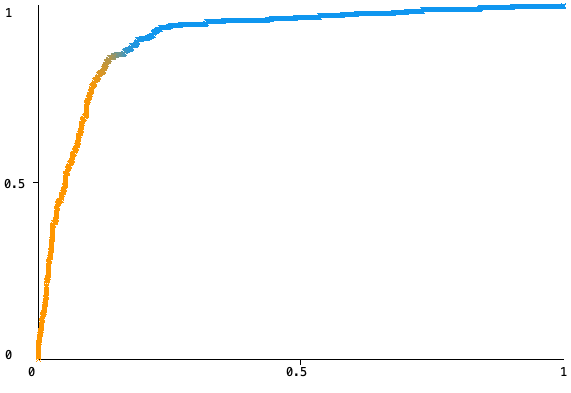
\includegraphics[width=8cm]{images/3_1_naive_bayes_suspect.png}
         \captionof{figure}{Naive Bayes (Suspect)}
     \end{minipage}
 \end{center}

 \subsubsection{k-NN}

 \begin{center}
     \begin{minipage}{0.48\linewidth}
         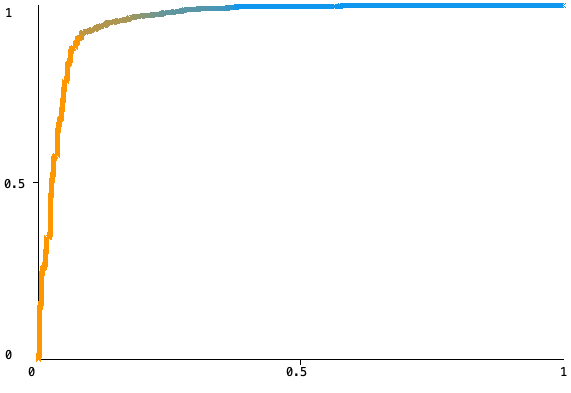
\includegraphics[width=8cm]{images/3_1_knn_normal.png}
         \captionof{figure}{k-NN (Normal)}
     \end{minipage}
     \begin{minipage}{0.48\linewidth}
         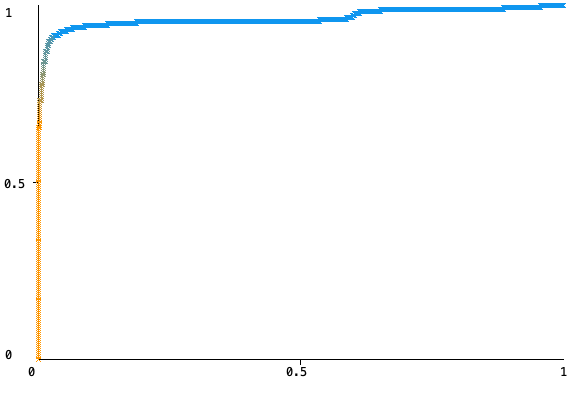
\includegraphics[width=8cm]{images/3_1_knn_pathological.png}
         \captionof{figure}{k-NN (Pathological)}
     \end{minipage}
     \begin{minipage}{0.48\linewidth}
         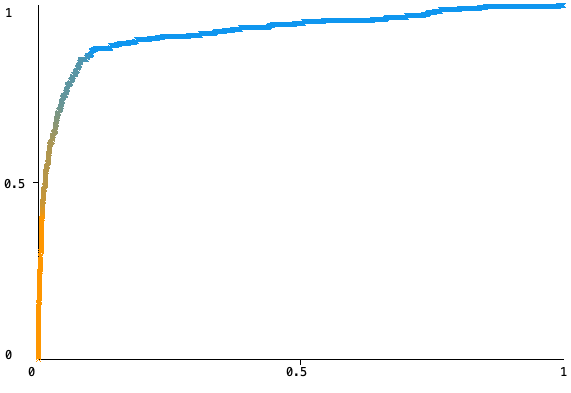
\includegraphics[width=8cm]{images/3_1_knn_suspect.png}
         \captionof{figure}{k-NN (Suspect)}
     \end{minipage}
 \end{center}

 \subsubsection{Decision Tree}

 \begin{center}
     \begin{minipage}{0.48\linewidth}
         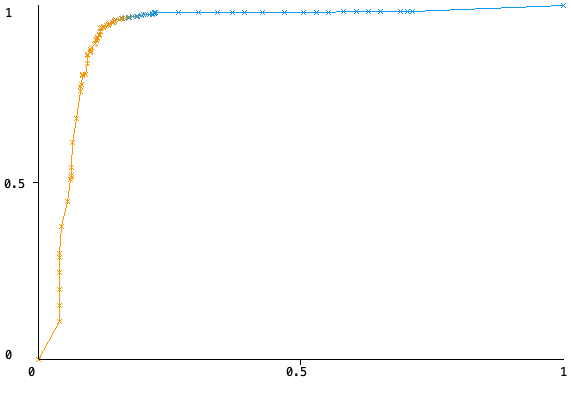
\includegraphics[width=8cm]{images/3_1_decision_tree_normal.png}
         \captionof{figure}{Decision Tree (Normal)}
     \end{minipage}
     \begin{minipage}{0.48\linewidth}
         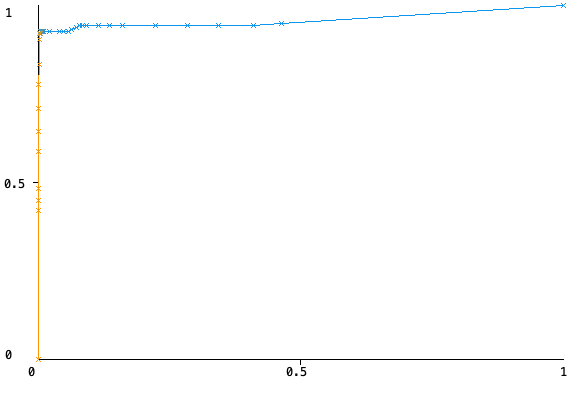
\includegraphics[width=8cm]{images/3_1_decision_tree_pathological.png}
         \captionof{figure}{Decision Tree (Pathological)}
     \end{minipage}
     \begin{minipage}{0.48\linewidth}
         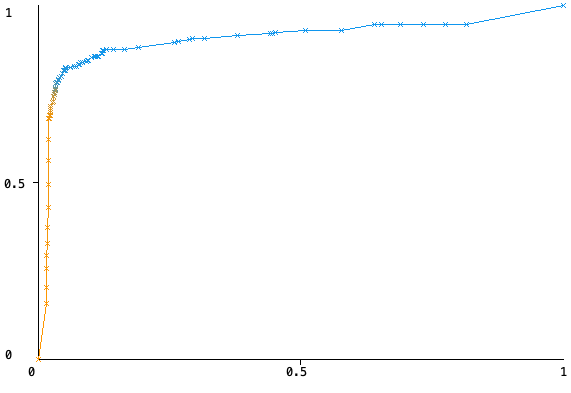
\includegraphics[width=8cm]{images/3_1_decision_tree_suspect.png}
         \captionof{figure}{Decision Tree (Suspect)}
     \end{minipage}
 \end{center}

 \subsection{Learnings from the ROC curves}
 Since ROC curves are plotted using the true positive rate (TPR) against the false positive rate (FPR), it
 helps us to visualize the performance of the classifiers at different thresholds and ideally we would want
 the curve to be above the "random" reference line and as close to the top left corner as possible because
 the top left corner represents the best case where $TPR = 1.0$ and $FPR = 0.0$ meaning the model has no
 false positive results. One way to measure this is by calculating the area under the ROC curve (AUC), the
 closer the AUC is to 1.0, the better the model is and for the curve to be above the "random" reference line,
 the AUC must be more than 0.5. From the ROC curves above, we can deduce the area under the ROC curve (AUC)
 for each classifier:

 \begin{center}
     \begin{tabular}{| c | c |}
         \hline
         \textbf{Classifier} & \textbf{Area under the ROC curve (AUC)}               \\ [0.5ex]
         \hline
         Naive Bayes         & 0.947 (Normal), 0.888 (Pathological), 0.907 (Suspect) \\
         \hline
         k-NN                & 0.957 (Normal), 0.962 (Pathological), 0.923 (Suspect) \\
         \hline
         Decision Tree       & 0.920 (Normal), 0.957 (Pathological), 0.903 (Suspect) \\
         \hline
     \end{tabular}
     \captionof{table}{Area under the ROC curve (AUC) for each classifier}
 \end{center}

 \subsection{Conclusion}
 Based on Table 5, we can see that the k-NN classifier has the highest AUC for all 3 classes and hence
 it is the best classifier among the 3. I am satisfied with the result because the k-NN classifier has AUC of more than 0.9
 for all 3 classes and this means that the classifier is able to classify the instances correctly most of the time. Note that the k-NN classifier was ran with the parameters:

 \begin{enumerate}
     \item $k = 3$
     \item $k$ fold-cross validation = 10
     \item 1/d weighting
 \end{enumerate}
\end{section}

\begin{section}{Most discriminating features}
 To find the most discriminating fetaures, I applied the \textbf{AttributeSelection} filter with \textbf{InfoGainAttributeEval}
 as the evaluator and \textbf{Ranker} as the search method in the preprocess tab. This filter sorts the features by their information
 gain compared to the class and the result is as follows:

 \begin{center}
     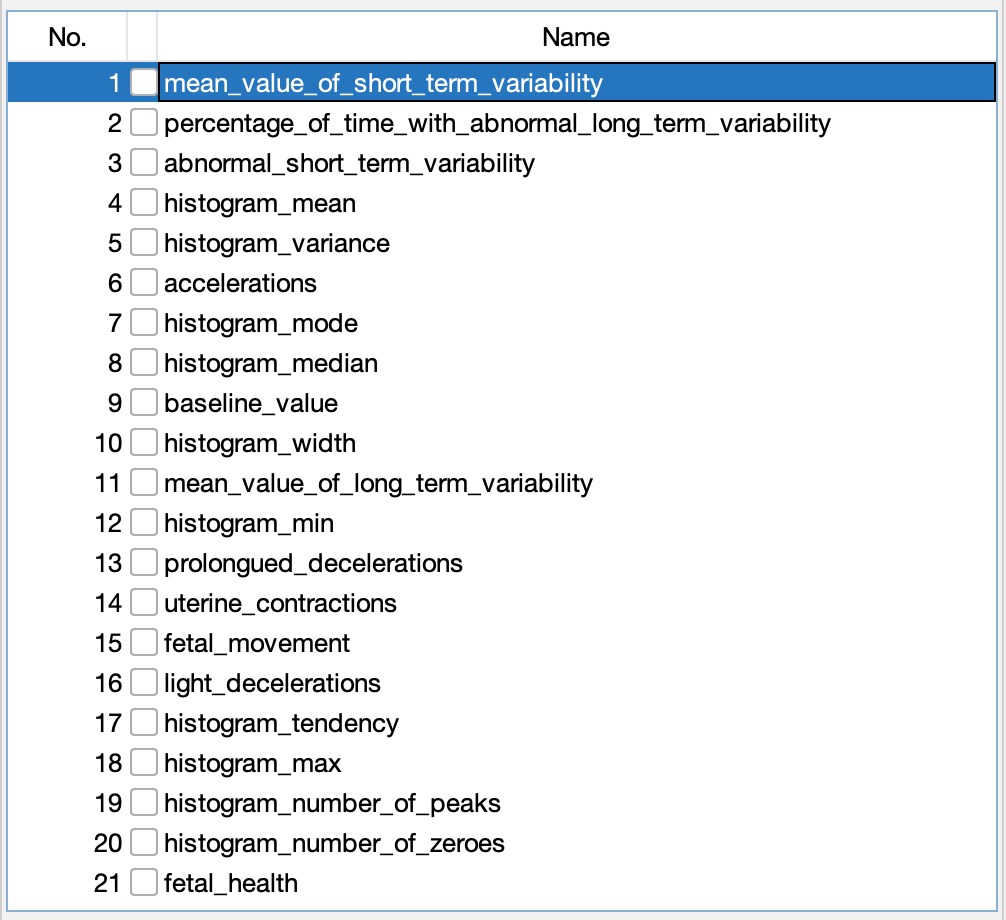
\includegraphics[width=10cm]{images/4_1_finding_most_discriminating_features.png}
     \captionof{figure}{Features sorted by information gain}
 \end{center}

 From the figure above, we can see that the top 5 most discriminating features are:
 \begin{enumerate}
     \item \textbf{mean\_value\_of\_short\_term\_variability}
     \item \textbf{percentage\_of\_time\_with\_abnormal\_long\_term\_variability}
     \item \textbf{abnormal\_short\_term\_variability}
     \item \textbf{histogram\_mean}
     \item \textbf{histogram\_variance}
 \end{enumerate}

\end{section}

\begin{section}{Finding the top 5 features}
 \subsection{Wrapper + Forward Search}
 To achieve this I used the \textbf{WrapperSubsetEval} attribute evaluator with J48 as the classifier and
 the search method \textbf{GreedyStepwise} with \texttt{searchBackwards = false}. The result is shown below.

 \begin{center}
     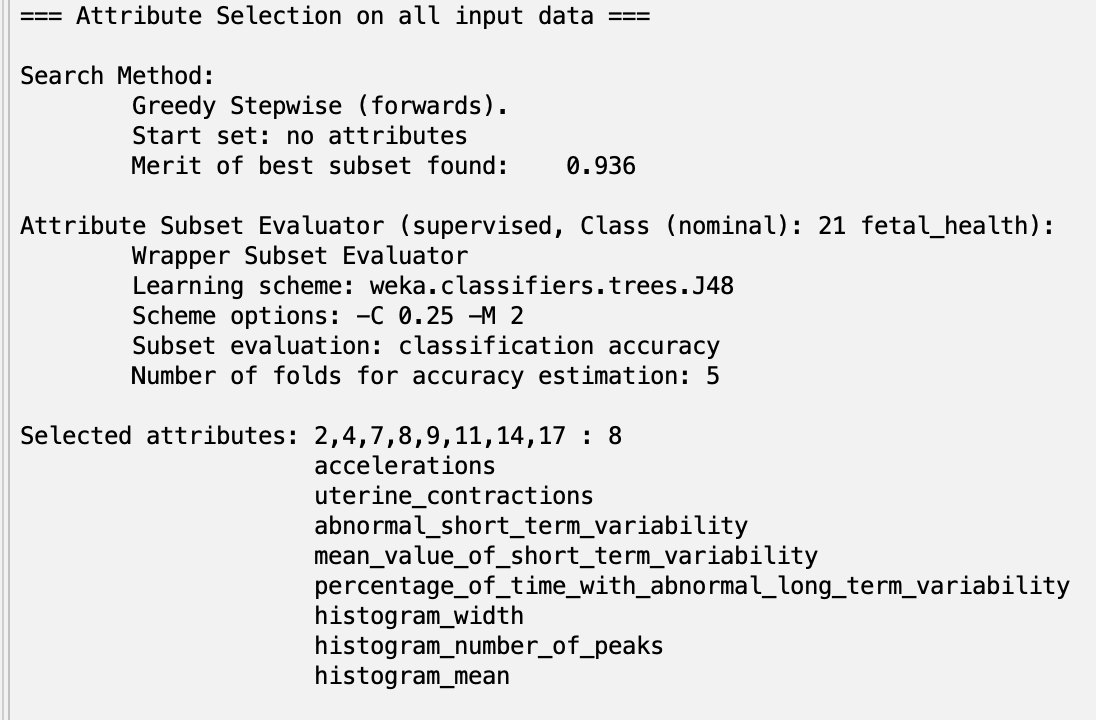
\includegraphics[width=12cm]{images/5_2_wrapper_forwards.png}
     \captionof{figure}{Wrapper + Forward Search feature selection}
 \end{center}

 \subsection{Wrapper + Backward Search}
 To achieve this I used the \textbf{WrapperSubsetEval} attribute evaluator with J48 as the classifier and
 the search method \textbf{GreedyStepwise} with \texttt{searchBackwards = true}. The result is shown below.

 \begin{center}
     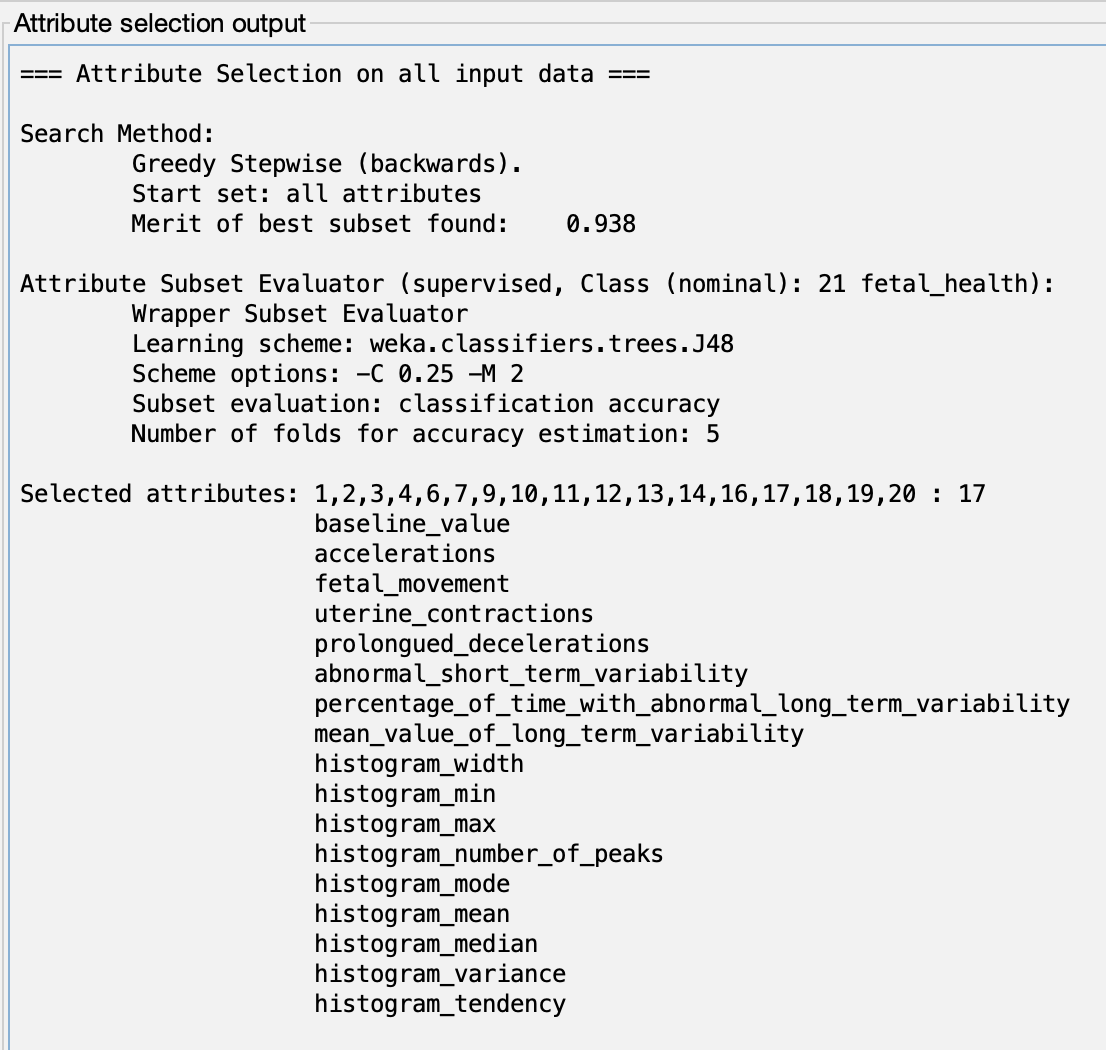
\includegraphics[width=12cm]{images/5_2_wrapper_backwards.png}
     \captionof{figure}{Wrapper + Backward Search feature selection}
 \end{center}

 \subsection{Information Gain}
 To achieve this I used the \textbf{InfoGainAttributeEval} attribute evaluator with
 the search method \textbf{Ranker}. The result is shown below.

 \begin{center}
     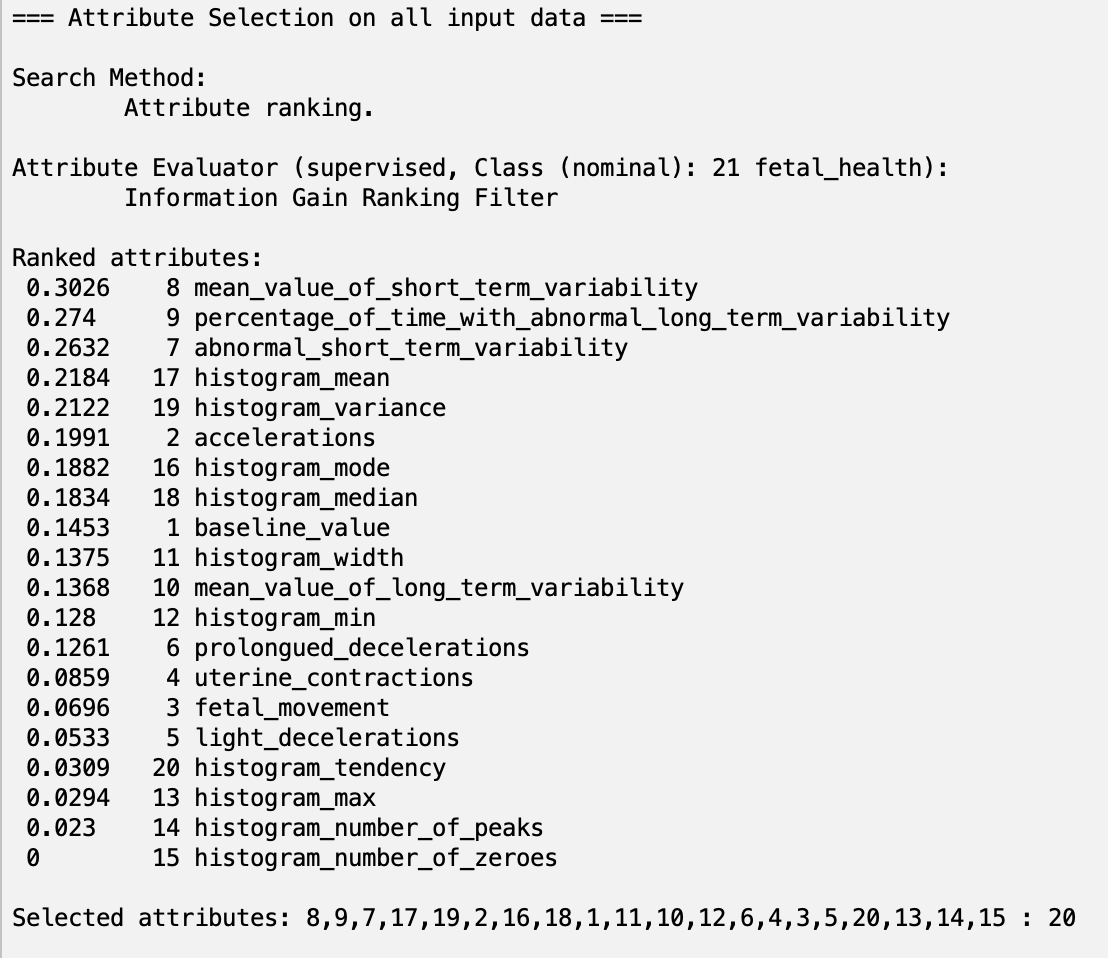
\includegraphics[width=12cm]{images/5_2_information_gain.png}
     \captionof{figure}{Information Gain feature selection}
 \end{center}

 \subsection{Discussion}
 By comparing the number of selected attributes from the three methods above, we can already see significant
 differences. \textit{Wrapper + Forward Search} selected only 8 attributes, \textit{Wrapper + Backward Search}
 selected 17 attributes and \textit{Information Gain} selected all 20 attributes. The information gain method
 merely ranks the attributes based on their information gain and does not select a subset of attributes hence
 resulting in all attributes being selected whereas the wrapper method uses a classifier to evaluate
 the attributes and select only the subset of features which has the most impact on the classifier's performance.
 Since forward search starts with an empty set and only adds attributes iteratively, it made sense that it selected
 lesser attributes than backward search which starts with all attributes and removes attributes iteratively.
\end{section}

\begin{section}{Classifier performance with the top 5 features}
 \subsection{Wrapper + Forward Search}
 The results was obtained by running the classifiers with the following 5 features:
 \begin{enumerate}
     \item \textbf{accelerations}
     \item \textbf{uterine\_contractions}
     \item \textbf{abnormal\_short\_term\_variability}
     \item \textbf{mean\_value\_of\_short\_term\_variability}
     \item \textbf{percentage\_of\_time\_with\_abnormal\_long\_term\_variability}
 \end{enumerate}

 \begin{center}
     \begin{tabular}{| c | c | c | c |}
         \hline
         \textbf{F1-Measure}       & \textbf{Naive Bayes} & \textbf{k-NN} & \textbf{Decision Tree} \\ [0.5ex]
         \hline
         \textbf{Normal}           & 0.889                & 0.941         & 0.940                  \\
         \hline
         \textbf{Pathologic}       & 0.105                & 0.766         & 0.729                  \\
         \hline
         \textbf{Suspect}          & 0.602                & 0.727         & 0.759                  \\
         \hline
         \hline
         \textbf{Weighted Average} & 0.785                & 0.897         & 0.897                  \\
         \hline
     \end{tabular}
     \captionof{table}{F1-Measure of each class using the top 5 features from Wrapper + Forward Search}
 \end{center}

 The average of the 3 weighted average F1-Measure is $0.860$.

 \subsection{Wrapper + Backward Search}
 The results was obtained by running the classifiers with the following 5 features:
 \begin{enumerate}
     \item \textbf{baseline\_value}
     \item \textbf{accelerations}
     \item \textbf{fetal\_movement}
     \item \textbf{uterine\_contractions}
     \item \textbf{prolongued\_decelerations}
 \end{enumerate}

 \begin{center}
     \begin{tabular}{| c | c | c | c |}
         \hline
         \textbf{F1-Measure}       & \textbf{Naive Bayes} & \textbf{k-NN} & \textbf{Decision Tree} \\ [0.5ex]
         \hline
         \textbf{Normal}           & 0.901                & 0.928         & 0.925                  \\
         \hline
         \textbf{Pathologic}       & 0.579                & 0.728         & 0.706                  \\
         \hline
         \textbf{Suspect}          & 0.572                & 0.584         & 0.563                  \\
         \hline
         \hline
         \textbf{Weighted Average} & 0.829                & 0.864         & 0.857                  \\
         \hline
     \end{tabular}
     \captionof{table}{F1-Measure of each class using the top 5 features from Wrapper + Backward Search}
 \end{center}

 The average of the 3 weighted average F1-Measure is $0.850$.

 \subsection{Information Gain}
 The results was obtained by running the classifiers with the following 5 features:
 \begin{enumerate}
     \item \textbf{mean\_value\_of\_short\_term\_variability}
     \item \textbf{percentage\_of\_time\_with\_abnormal\_long\_term\_variability}
     \item \textbf{abnormal\_short\_term\_variability}
     \item \textbf{histogram\_mean}
     \item \textbf{histogram\_variance}
 \end{enumerate}

 \begin{center}
     \begin{tabular}{| c | c | c | c |}
         \hline
         \textbf{F1-Measure}       & \textbf{Naive Bayes} & \textbf{k-NN} & \textbf{Decision Tree} \\ [0.5ex]
         \hline
         \textbf{Normal}           & 0.908                & 0.953         & 0.952                  \\
         \hline
         \textbf{Pathologic}       & 0.605                & 0.852         & 0.870                  \\
         \hline
         \textbf{Suspect}          & 0.584                & 0.712         & 0.768                  \\
         \hline
         \hline
         \textbf{Weighted Average} & 0.838                & 0.912         & 0.920                  \\
         \hline
     \end{tabular}
     \captionof{table}{F1-Measure of each class using the top 5 features from Wrapper + Backward Search}
 \end{center}

 The average of the 3 weighted average F1-Measure is $0.890$.

 \subsection{Discussion}
 By comparing the results above, we can see that the top 5 features from \textit{Information Gain} performed
 the best and I think this is due to the fact that information gain uses filters and filters has no feature
 dependencies and no model bias. Looking at the two wrapper methods, forward search performed slightly better
 than backward search on average but it performed very poorly in the \textit{Pathologic} class of \textit{Naive Bayes},
 I think the reason for this is that one of the dominating feature for this specific class was not included in the
 top 5 features.
\end{section}

\section{Principal Components}
\subsection{Extracting Principal Components}
I used the \textbf{PrincipalComponents} filter with \texttt{centerData = true} in the preprocess tab to combine existing
features into principal components. I then removed the other features from the third ranked to the last ranked so I
was left with two features. The result looks like this:

\begin{center}
    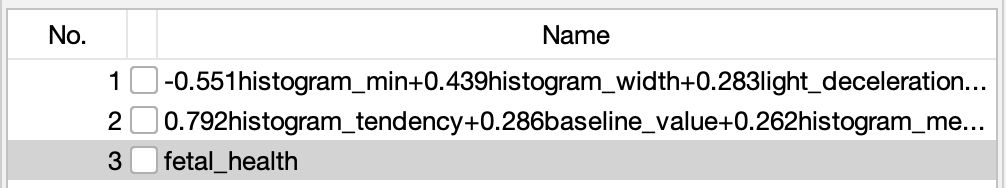
\includegraphics[width=12cm]{images/7_1_preprocess_principal_components.png}
    \captionof{figure}{Principal components}
\end{center}

\subsection{Classifiers performance using the principal components}

\begin{center}
    \begin{tabular}{| c | c | c | c |}
        \hline
        \textbf{F1-Measure}       & \textbf{Naive Bayes} & \textbf{k-NN} & \textbf{Decision Tree} \\ [0.5ex]
        \hline
        \textbf{Normal}           & 0.902                & 0.907         & 0.914                  \\
        \hline
        \textbf{Pathologic}       & 0.344                & 0.680         & 0.685                  \\
        \hline
        \textbf{Suspect}          & 0.344                & 0.471         & 0.452                  \\
        \hline
        \hline
        \textbf{Weighted Average} & 0.779                & 0.828         & 0.831                  \\
        \hline
    \end{tabular}
    \captionof{table}{F1-Measure of each class and weighted average using principal components}
\end{center}

The average of the 3 weighted average F1-Measure is $0.813$. Comparing this to the results from the previous section,
we can see that the performance of the classifiers dropped significantly. This is because although applying principal
component analysis (PCA) reduces the dimensionality of the dataset, it also reduces the variance in the dataset. Therefore,
the classifiers are not able to perform as well as before.

\subsection{Principal Components Visualisation}

\begin{center}
    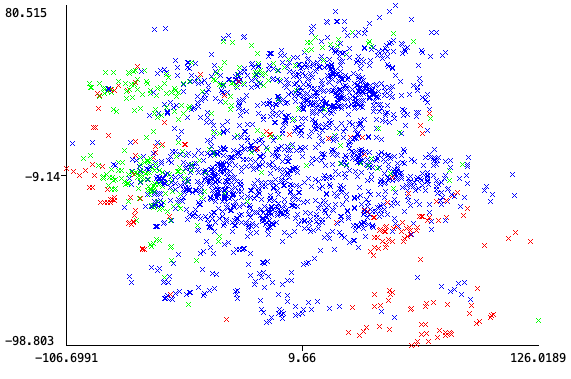
\includegraphics[width=14cm]{images/7_1_principal_components.png}
    \captionof{figure}{Principal components visualisation}
\end{center}

In the visualisation above, \textbf{Normal} is represented by blue, \textbf{Pathologic} is represented by red and \textbf{Suspect}
is represented by green.

\subsection{Expectation}
In my opinion, it is expected that just by doing PCA alone the performance of the classifiers would drop compared to feature selection
such as \textit{Information Gain}. This is because even PCA preserves most of the variance in the dataset, it does not take into account
which features are more important than others. Therefore, the classifiers would not be able to perform as well as before. Perhaps if we do
PCA with more components and followed by feature selection, then the performance of the classifiers would be on par or better.

\end{document}